The Quick Responce (QR) Code was announced in 1994. Having been under development for several years at Denso Wave, barcode developer, the goal was to create a new form of barcode that could carry more information and be easily read.\cite{qrCodeHistory}

	\begin{figure}[ht!]
		\centering
		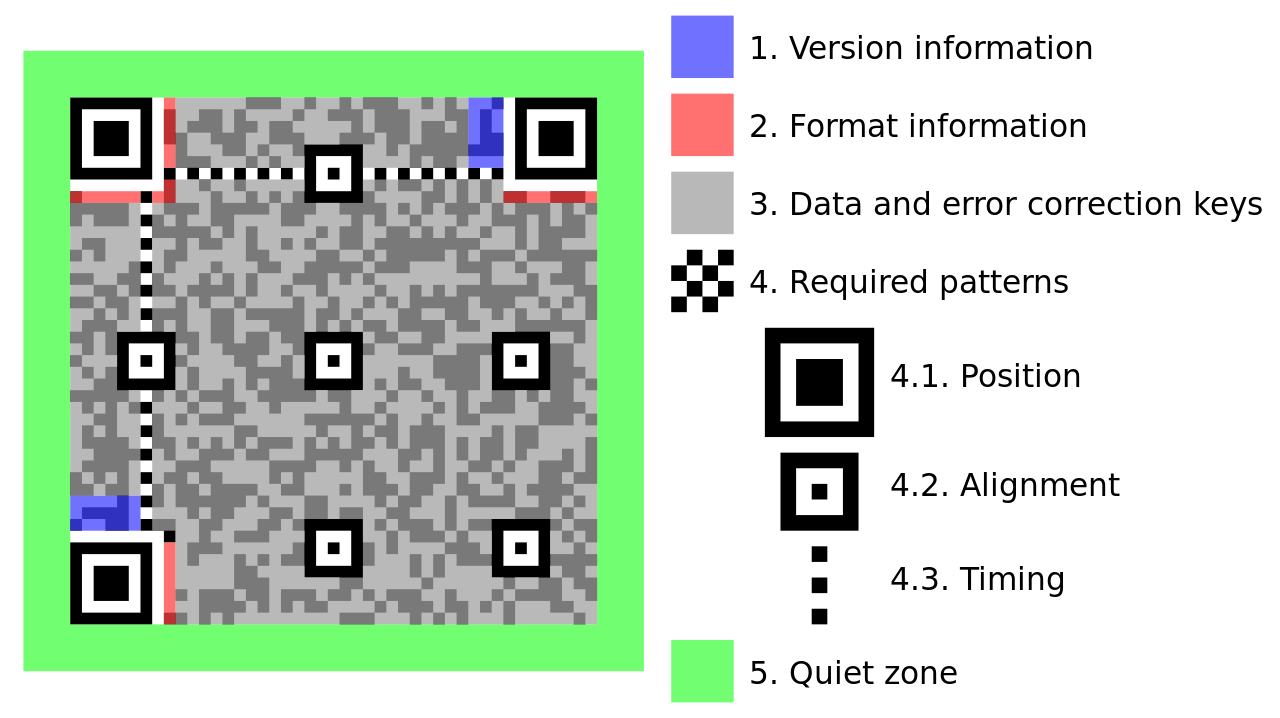
\includegraphics[width=110mm]{images/qrcodestandard}
		\caption{The standardised fields in a QR Code.\cite{qrCodeWiki}}
		\label{qrcodestandard}
	\end{figure}
	
[TODO WRITE ABOUT THE STANDARDISED FIELDS OF QR CODE]